\documentclass[12pt,a4paper]{article}
\usepackage{pgf}
\usepackage{svg}
\usepackage{tikz}
\usepackage{stanli}
\usepackage{afterpage}
\usepackage{multirow}
\usepackage{subfig}
\usepackage{pgfpages}
\usepackage{rotating}
\usepackage[english]{babel}
\usepackage[a4paper,top=2cm,bottom=1.5cm,left=1.5cm,right=1.5cm,marginparwidth=1.75cm]{geometry}
\usepackage{amsmath}
\usepackage{graphicx}
\usepackage[colorlinks=true, allcolors=blue]{hyperref}

\title{}
\author{}
\date{}

\begin{document}
    \begin{titlepage}
    \begin{center}
        \Huge
        \textbf{F1 engine cylinder sound classification with FFT and Deep Learning}
        
        
        \vspace{7cm}
        
        
\includegraphics[width=0.4\textwidth]{images/its-logo.png}
        
    \end{center}
        \vspace{5cm}
    \Large
    \begin{tabbing}
        \hspace*{1em}\= \hspace*{8em} \= \kill % set the tabbings
        \> Name:\>  \textbf{Ikhwanul Abiyu Dhiyya'ul Haq} \\
        \> NRP:\>  5024211048 \\
        \> Lecturer:\>  Dion Hayu Fandiantoro, S.T.,M.T.  \\
        \> Subject:\>  Digital Signal Processing  \\
    \end{tabbing}

\end{titlepage}

% 
    \begin{center}
    \Large
    \textbf{Table of Contents\\}
\end{center}

\renewcommand{\contentsname}{}
\tableofcontents{}

\newpage
    \section{Pendahuluan}
\subsection{Latar belakang}

Kemajuan teknologi otomotif telah mengarah pada pengembangan mesin berperforma tinggi, khususnya di balap Formula 1 (F1). Suara khas yang dihasilkan oleh mesin F1 memainkan peran penting baik dalam analisis performa maupun pengalaman penonton. Kemampuan untuk mengklasifikasikan dan menganalisis suara mesin secara akurat dapat memberikan wawasan berharga untuk diagnostik mesin, pengoptimalan performa, dan bahkan meningkatkan pengalaman balap secara keseluruhan. \newline

Metode klasifikasi suara tradisional sering mengandalkan inspeksi manual dan penilaian subjektif, yang dapat memakan waktu dan rentan terhadap kesalahan. Dalam beberapa tahun terakhir, penerapan teknik pemrosesan sinyal digital dan algoritma pembelajaran mesin telah menunjukkan hasil yang menjanjikan dalam mengotomatiskan klasifikasi dan analisis suara mesin. \newline

\textit{Fast Fourier Transform} (FFT) adalah teknik pemrosesan sinyal yang banyak digunakan yang memungkinkan kita menganalisis komponen frekuensi dari sinyal suara yang diberikan. Dengan mentransformasi bentuk gelombang suara dari domain waktu ke domain frekuensi, kita dapat mengekstrak fitur penting yang mencirikan suara mesin, seperti komponen frekuensi dominan dan struktur harmonik. \newline

\textit{Deep Learning}, subbidang pembelajaran mesin, telah mendapatkan perhatian yang signifikan karena kemampuannya untuk secara otomatis mempelajari representasi hierarkis dari data yang kompleks. \textit{Convolutional Neural Networks} (CNNs), sejenis model pembelajaran mendalam, telah menunjukkan performa luar biasa dalam berbagai tugas klasifikasi audio. Dengan memanfaatkan CNN, kami dapat membangun sistem klasifikasi suara mesin yang kuat dan akurat yang dapat membedakan antara kondisi dan kondisi mesin yang berbeda berdasarkan fitur frekuensi yang diekstraksi. \newline

Dalam penelitian ini, kami bertujuan untuk mengembangkan sistem klasifikasi suara untuk suara silinder mesin F1 menggunakan kombinasi FFT dan teknik deep learning. Dengan menganalisis konten frekuensi suara mesin dan melatih model CNN pada kumpulan data besar sampel suara mesin berlabel, kami berupaya mencapai akurasi klasifikasi tinggi dan performa waktu nyata. Sistem yang diusulkan memiliki potensi untuk membantu insinyur balap, mekanik, dan penggemar balap dalam mendiagnosis masalah mesin, memantau kinerja, dan meningkatkan pengalaman balap F1 secara keseluruhan.

\subsection{Rumusan masalah}

Berdasarkan latar belakang di atas, maka kami merumuskan masalah sebagai berikut:

\begin{enumerate}
    \item Bagaimana peran FFT dalam pemrosesan sinyal suara?
    \item Bagaimana algoritma \textit{deep learning} yang optimal untuk melakukan klasifikasi suara?
    \item Bagaimana hasil dari berbagai metode \textit{deep learning} mempengaruhi output dari program?
\end{enumerate}

\subsection{Tujuan Penelitian}

Tujuan dari dilakukannya penelitian ini adalah sebagai berikut:

\begin{enumerate}
    \item Mengetahui peran FFT dalam pemrosesan sinyal suara.
    \item Mengetahui algoritma \textit{deep learning} yang optimal dalam melakukan klasifikasi suara
    \item Mengetahui hasil dari berbagai metode \textit{deep learning} dan pengaruhnya terhadap output program
\end{enumerate}

\subsection{Manfaat}

Manfaat yang bisa diberikan oleh penelitian ini adalah bisa menjadi sumber pembelajaran dan bahan bacaan untuk penelitian penelitian lain tentang pemrosesan sinyal dan \textit{Deep Learning} 

\subsection{Metode Penelitian}

Metode yang digunakan untuk penelitian ini yaitu metode kuantitatif, dengan mengambil dataset suara dari \textit{YouTube} berupa suara-suara \textit{onboard camera} dari berbagai musim di F1. Yang kemudian dataset tersebut di-\textit{program} menggunakan bahasa pemrograman \textit{python}

\newpage
    \section{Tinjauan Pustaka}
\subsection{Konsep Dasar Suara Silinder Mesin F1}
\subsubsection{Komponen-komponen penting pada mesin F1}

Mesin F1 (Sering disebut \textit{Power Unit}) F1 saat ini menggunakan beberapa elemen: \textit{Internal Combustion Engine} (ICE), \textit{Motor Generator Unit-Heat} (MGU-H), \textit{Motor Generator Unit-Kinetic} (MGU-K), \textit{Turbocharger} (TC), \textit{energy store} (ES), \textit{Control Electronic} (CE) dan knalpot. \newline

Pada ICE terjadi proses pembakaran dimana bahan bakar dan udara dicampur dan dinyalakan untuk membebaskan energi. Proses ini bekerja dengan cara yang sama seperti pada mobil jalan, namun, sistemnya sedikit lebih rumit. \newline

Jika dilihat lebih detail, udara hasil pembakaran dialirkan ke mesin melalui saluran udara yang berada di belakang roll hoop. Tekanan udara dinaikkan oleh kompresor yang merupakan bagian dari turbocharger. \newline

\begin{figure}[htbp]
    \centering
    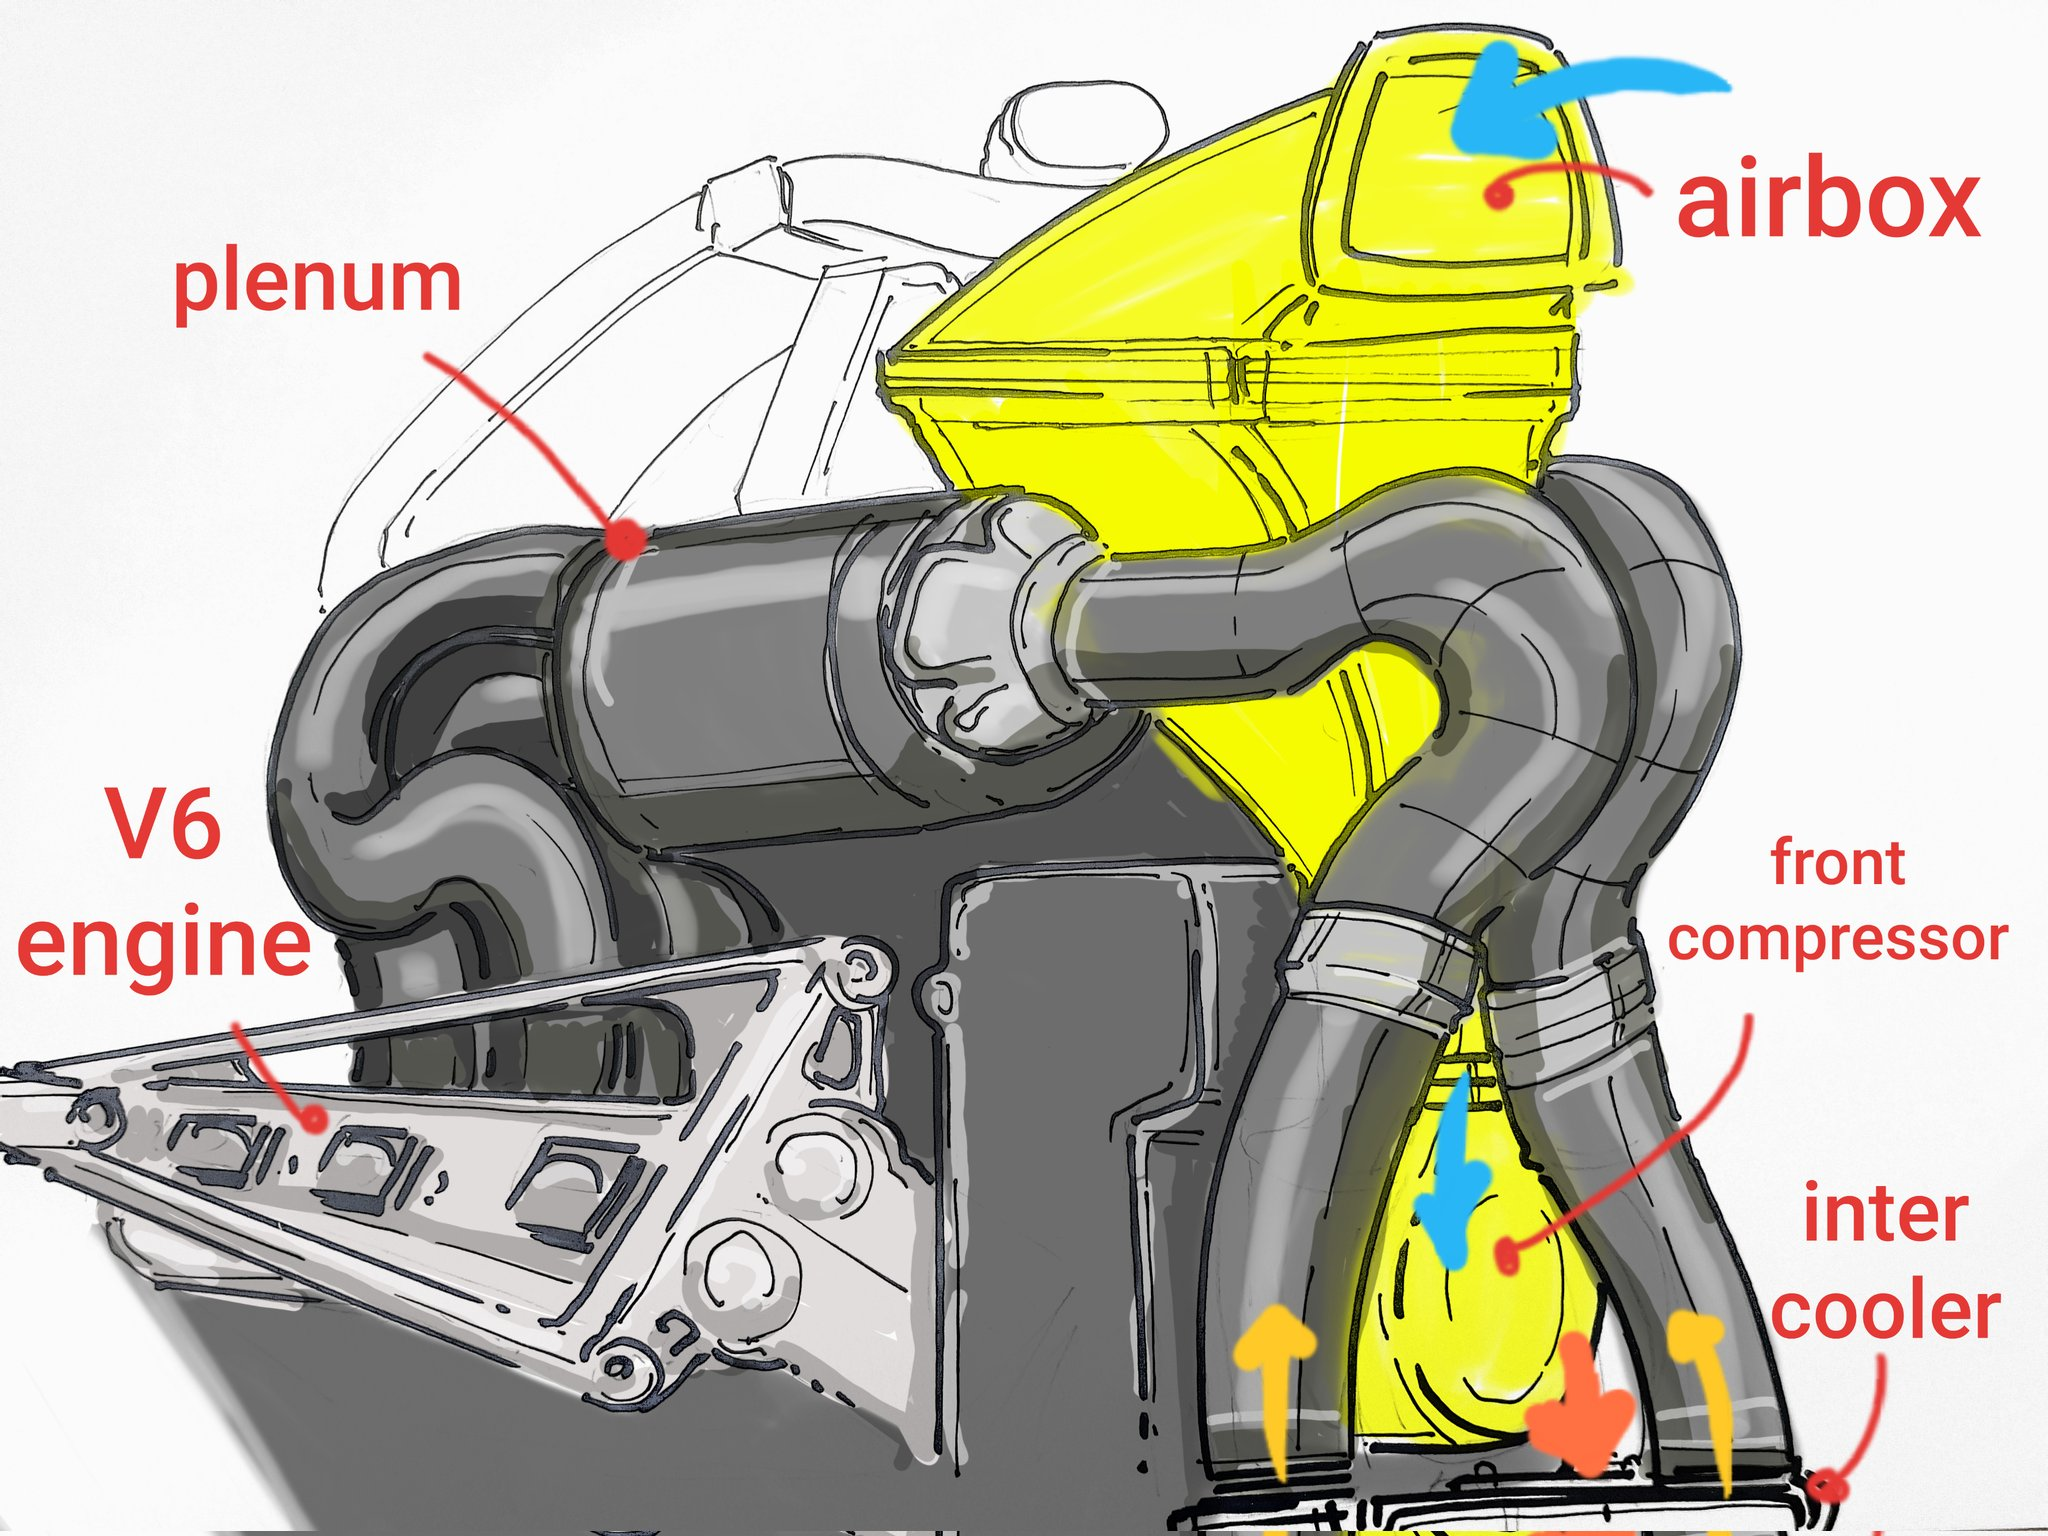
\includegraphics[width=0.8\textwidth]{images/f1-engine.jpg}
    \caption{Proses pembakaran pada ICE}
    \label{fig:Proses pembakaran pada ICE}
\end{figure}

Proses ini juga meningkatkan suhu udara, sehingga udara perlu didinginkan kembali dalam pendingin muatan sebelum dimasukkan ke dalam plenum di bagian atas mesin. \newline

Dari sana, ia melewati enam lubang saluran masuk dan melewati dua katup saluran masuk ke dalam silinder. Di situlah bahan bakar mulai berlaku. \newline

Mesin F1 injeksi langsung, seperti kebanyakan mobil jalan modern, sehingga bahan bakar disuntikkan langsung ke ruang bakar. \newline

Bahan bakar diinjeksikan maksimal 500 bar, yang dibatasi oleh regulasi. Meskipun itu lebih dari yang kita temukan pada mesin bensin injeksi langsung di mobil jalan raya, yang biasanya melihat tekanan hingga 350 bar, ini sebenarnya sedikit lebih sedikit daripada yang mungkin kita temukan di diesel modern, di mana tekanan bahan bakar bisa. mencapai hingga 2.500 bar. \newline

Campuran udara dan bahan bakar dikompresi oleh piston sebelum busi menyalakannya. Kekuatan pembakaran menekan piston, yang terhubung ke poros engkol melalui batang penghubung dan, oleh karena itu, mampu menggerakkan poros engkol. \newline

Saat piston naik kembali, katup buang terbuka untuk melepaskan gas buang dari mesin, sehingga seluruh proses dapat dimulai dari awal lagi – hingga maksimum 15.000 kali setiap menit (atau hingga 250 kali per detik). \newline

Gas buang digunakan untuk menggerakkan roda turbin turbocharger yang pada gilirannya menggerakkan kompresor. Apa yang tersisa kemudian keluar melalui knalpot di bagian belakang mobil, dengan sistem wastegate digunakan untuk mengontrol tekanan selama fase ini.

\subsubsection{Sistem knalpot dan pengaruhnya terhadap suara silinder}

Keluarnya gas buang dimulai setelah pembakaran terjadi. Kemudian, selama langkah buang saat piston bergerak kembali ke atas silinder, katup buang terbuka dan gas yang terbakar dikeluarkan dari ruang bakar. Gas kemudian berjalan ke satu set primer atau header, dengan satu primer per silinder (\textcolor{red}{merah}, \textcolor{purple}{ungu}, \textcolor{blue}{biru}). Tiga primer yang berasal dari masing-masing tepi mesin kemudian bergabung bersama dalam kolektor primer tiga-ke-satu (\textcolor{orange}{orange}) dan kemudian pipa sekunder (\textcolor{yellow}{kuning}). Dua sekunder (satu dari setiap sisi mesin) kemudian masuk ke turbocharger.

\begin{figure}[htbp]
    \centering
    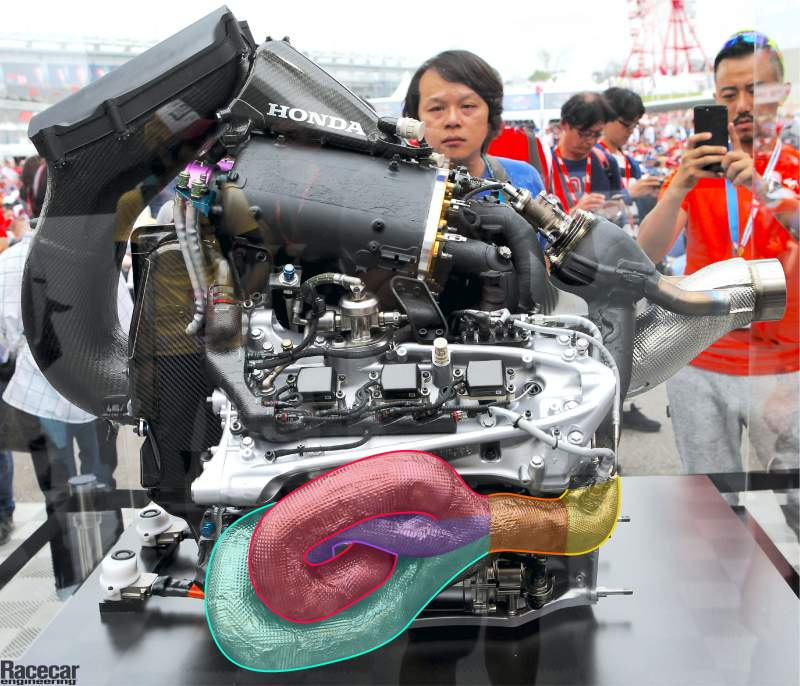
\includegraphics[width=0.7\textwidth]{images/F1-Exhaust-primaries_Honda_RA618H.jpg}
    \caption{Primer (\textcolor{red}{merah}, \textcolor{purple}{ungu}, \textcolor{blue}{biru}), kolektor (\textcolor{orange}{orange}) dan sekunder (\textcolor{yellow}{kuning}) pada \textit{power unit} Honda RA618H 2018}
    \label{fig:The primaries (red, purple, blue), collector (orange) and secondaries (yellow) on the 2018 Honda RA618H power unit}
\end{figure}

Bergantung pada pabrikan mesin, primer, kolektor, dan sekunder dapat menjadi satu bagian dan diintegrasikan ke dalam turbocharger, atau bagian terpisah. Knalpot (\textcolor{blue}{biru}) dari turbocharger kemudian membawa gas buang dari turbo ke bagian belakang mobil. Sementara ada juga wastegate yang mengontrol kecepatan turbo dan terdiri dari satu atau dua pipa wastegate (\textcolor{red}{merah}) yang keluar dari sekunder dan melewati rumah turbin, keluar di bagian belakang mobil.

\begin{figure}[htbp]
    \centering \footnotesize
    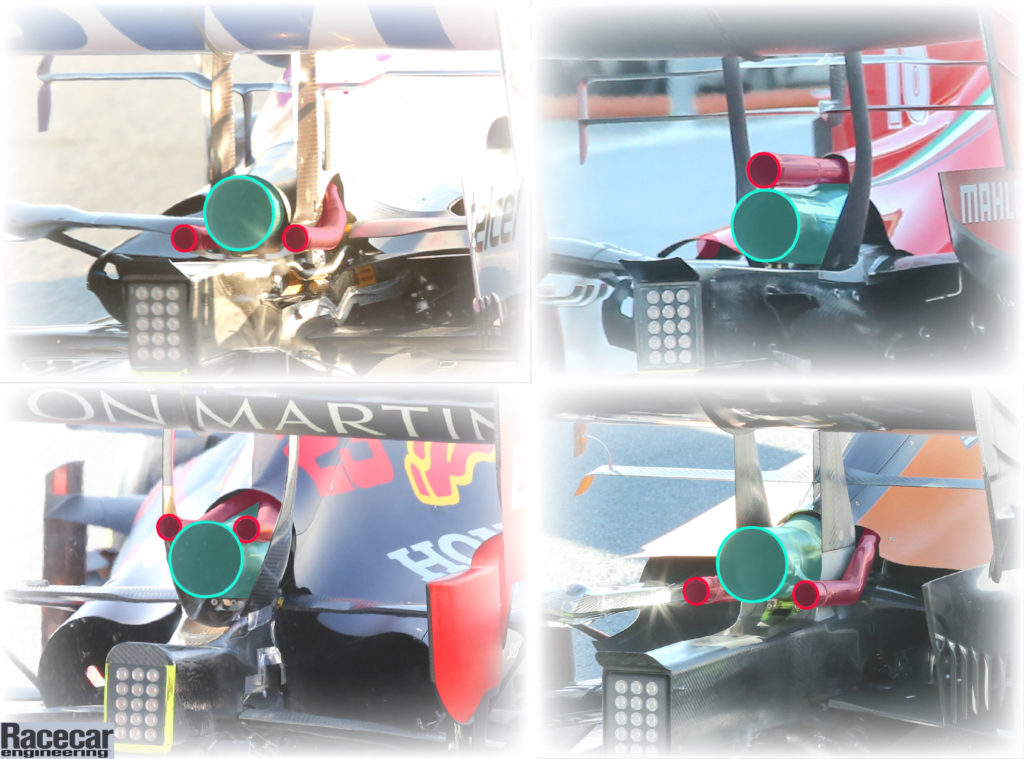
\includegraphics[width=0.7\textwidth]{images/F1-Exhaust-tailpipe-comparison-1024x759.jpg}
    \caption{Tata letak knalpot (\textcolor{blue}{biru}) dan wastegate (\textcolor{red}{merah}) dari empat \textit{power unit} yang berbeda. Kiri atas: Mercedes (Racing Point RP20). Kanan atas: Ferrari SF1000. Kiri bawah: Honda (Red Bull RB16). Kanan bawah: Renault (McLaren MCL35) (Sumber : https://www.racecar-engineering.com) }
    \label{fig:The tailpipe (blue) and wastegate (red) layouts of the four different power units. Top left: Mercedes (Racing Point RP20). Top right: Ferrari SF1000. Bottom left: Honda (Red Bull RB16). Bottom right: Renault (McLaren MCL35)}
\end{figure}

Meskipun konsep sistem pembuangan tampak relatif sederhana, ada banyak ilmu di balik parameter seperti panjang pipa, diameter, dan tata letak yang dapat dimanipulasi untuk menyetel torsi dan pita daya mesin.

\subsubsection{Karakteristik suara silinder pada mesin F1}

Mesin F1 dapat memiliki berbagai konfigurasi jumlah silinder, seperti V6TH (Turbo Hybrid), V8, V10, atau V12, tergantung pada peraturan yang berlaku pada saat tersebut. Umumnya, mesin dengan jumlah silinder yang lebih besar, seperti V10 atau V12, cenderung menghasilkan suara yang lebih berat, dalam hal volume dan kekayaan harmonik. Mesin dengan jumlah silinder yang lebih sedikit, seperti V6TH (Turbo Hybrid), cenderung menghasilkan suara yang lebih ringan atau teredam, tetapi dapat mencapai tingkat revolusi mesin yang lebih tinggi dan suara yang lebih tajam.

\subsection{Klasifikasi Suara Menggunakan FFT dan Deep Learning}
\subsubsection{Pengenalan tentang analisis Fourier Transform (FFT)}

TBA

\subsubsection{Penerapan FFT pada analisis suara silinder}

TBA

\subsubsection{Peran Deep Learning dalam klasifikasi suara}

TBA

\newpage
    \section{Metode Penelitian}

\subsection{Pengumpulan Data}

Pengumpulan dataset peneliti lakukan dengan mengambil kamera \textit{onboard} dari \textit{youtube}. Nantinya video tersebut akan peneliti ubah ke format .wav agar memudahkan pemrosesan olah suara, karena .wav merupakan file yang masih \textit{raw}, yaitu masih belum banyak diproses seperti .mp3 sehingga masih ada sedikit \textit{noise} yang terdengar 

\subsection{Praproses Data}

Data .wav ini nantinya akan kita proses menggunakan filter band-pass dan FFT sehingga suara noise seperti \textit{kerbs} bisa tereduksi dan pendengar bisa mendengar suara pure dari mesin dan knalpotnya saja.  

\subsection{Pelatihan Model Deep Learning}

TBA

\subsection{Evaluasi dan Validasi Model}

TBA

\newpage
    \section{Hasil dan Analisis}

\subsection{Deskripsi Dataset}

\subsubsection{Jumlah data suara yang terkumpul}

Jumlah suara yang terkumpul saat ini merupakan seluruh \textit{onboard pole position} dari Formula 1 musim 2018 (Masih Update)

\subsubsection{Karakteristik dataset yang digunakan}

Dataset nantinya akan menggunakan suara \textit{onboard} dari mesin V8 yang dipakai pada era 2006 - 2013, V10 dari tahun 1996 - 2005, dan V12 pada sebelum tahun 1995.

\subsection{Hasil Klasifikasi}

\subsubsection{Performa model dalam mengklasifikasikan suara silinder}

TBA

\subsubsection{Analisis hasil klasifikasi berdasarkan kategori suara}

TBA

\newpage
    \section{Kesimpulan}

\subsection{Ringkasan Temuan Penelitian}

TBA

\subsection{Implikasi Penelitian}

TBA

\subsection{Keterbatasan Penelitian}

TBA

\newpage
    \section{Saran}

\subsection{Rekomendasi untuk penelitian selanjutnya}

TBA

\subsection{Saran untuk pengembangan metode}

TBA

\newpage
    \section{Daftar Pustaka}

\begin{enumerate}
    \item \footnotesize\url{https://www.formula1.com/en/latest/article.the-beginners-guide-to-formula-1-engine-and-gearbox-penalties.2TSy7BFgEvdNLojGLWS3F1.html}
    \item \footnotesize\url{https://f1chronicle.com/how-a-formula-1-internal-combustion-engine-works/}
    \item \footnotesize\url{https://www.racecar-engineering.com/tech-explained/how-f1-exhausts-work/}
\end{enumerate}

    \nocite{*}
    \bibliography{content/references}
    
\end{document}
